\chapter{Kravspecifikation}

%% indledning til kapitel skal være her...
I de følgende afsnit vil der redegøres for kravspecifikationen, som indeholder de individuelle krav til projektet. 
Kravspecifikationen har til formål, at specificere hvad projektet skal omhandle ud fra de ønsker, 
projektgruppen og universitet har fremsat.

\section{Funktionelle krav}
Funktionelle krav for systemet er udviklet vha. \gls{us}\footnote{\url{http://www.agilemodeling.com/artifacts/userStory.htmlIntroduction}}.
I tabellen er  \gls{moscow}\footnote{\url{https://en.wikipedia.org/wiki/MoSCoW_method}} analysen skrevet ind. MoSCoW er udarbejdet efter principperne bag \gls{moscow}, som er en prioriteringsteknik brugt i projektstyring.

\begin{table}[H]
	\centering
	\begin{tabularx}{\linewidth}{|l|X|r|}
	\hline
	\rowcolor[HTML]{FFFFFF} 
	{\color[HTML]{000000} Type}                                                                              & {\color[HTML]{000000} User Story}                                                                                                                                     & {\color[HTML]{000000} MoSCoW} \\ \hline
	\multicolumn{1}{|l|}{\cellcolor[HTML]{FFFFFF}{\color[HTML]{000000} }}                                    & Som bruger vil jeg kunne tilgå systemet via et Windows PC program.                                                                                                    & Must                          \\ \cline{2-3} 
	\multicolumn{1}{|l|}{\cellcolor[HTML]{FFFFFF}{\color[HTML]{000000} }}                                    & Som bruger vil jeg kunne tilgå systemet via en iOS App.                                                                                                               & Could                         \\ \cline{2-3} 
	\multicolumn{1}{|l|}{\multirow{-3}{*}{\cellcolor[HTML]{FFFFFF}{\color[HTML]{000000} Deployment}}}        & Som bruger vil jeg kunne tilgå systemet fra enhjemmeside, for ikke at være afhængig af platform.                                                                      & Could                         \\ \hline
	\multicolumn{1}{|l|}{\cellcolor[HTML]{FFFFFF}{\color[HTML]{000000} }}                                    & \begin{tabular}[c]{@{}l@{}}Som bruger vil jeg kunne logge ud af systemet\\ for at afslutte adgang til mine data.\end{tabular}                                         & Should                        \\ \cline{2-3} 
	\multicolumn{1}{|l|}{\cellcolor[HTML]{FFFFFF}{\color[HTML]{000000} }}                                    & \begin{tabular}[c]{@{}l@{}}Som bruger vil jeg kunne nulstille mit kodeord,\\ hvis jeg skulle glemme det.\end{tabular}                                                 & Could                         \\ \cline{2-3} 
	\multicolumn{1}{|l|}{\cellcolor[HTML]{FFFFFF}{\color[HTML]{000000} }}                                    & \begin{tabular}[c]{@{}l@{}}Som uvedkommende vil jeg låses ude af systemet,\\ hvis jeg taster koden forkert, for ikke at få adgang til systemet.\end{tabular} & Could                         \\ \cline{2-3} 
	\multicolumn{1}{|l|}{\cellcolor[HTML]{FFFFFF}{\color[HTML]{000000} }}                                    & \begin{tabular}[c]{@{}l@{}}Som bruger vil jeg kunne sende en\\ ’tilladelse’ til andre brugere, så de kan se data om min pool.\end{tabular}                            & Could                         \\ \cline{2-3} 
	\multicolumn{1}{|l|}{\cellcolor[HTML]{FFFFFF}{\color[HTML]{000000} }}                                    & \begin{tabular}[c]{@{}l@{}}Som bruger vil jeg kunne ændre mit password for\\ at sikre min konto.\end{tabular}                                                         & Could                         \\ \cline{2-3} 
	\multicolumn{1}{|l|}{\multirow{-3}{*}{\cellcolor[HTML]{FFFFFF}{\color[HTML]{000000} Safety}}}            & \begin{tabular}[c]{@{}l@{}}Som bruger vil jeg have min data i systemet\\ krypteret.\end{tabular}                                                                      & Won't                         \\ \hline
	\multicolumn{1}{|l|}{\cellcolor[HTML]{FFFFFF}{\color[HTML]{000000} }}                                    & \begin{tabular}[c]{@{}l@{}}Som bruger vil jeg kunne oprette mig i systemet,\\ for at få adgang til systemet\end{tabular}                                              & Must                          \\ \cline{2-3} 
	\multicolumn{1}{|l|}{\cellcolor[HTML]{FFFFFF}{\color[HTML]{000000} }}                                    & \begin{tabular}[c]{@{}l@{}}Som bruger vil jeg kunne logge ind i systemet\\ for at se mine data.\end{tabular}                                                          & Must                          \\ \cline{2-3} 
	\multicolumn{1}{|l|}{\cellcolor[HTML]{FFFFFF}{\color[HTML]{000000} }}                                    & \begin{tabular}[c]{@{}l@{}}Som bruger vil jeg kunne tilføje en pool til min\\ konto.\end{tabular}                                                                     & Must                          \\ \cline{2-3} 
	\multicolumn{1}{|l|}{\cellcolor[HTML]{FFFFFF}{\color[HTML]{000000} }}                                    & \begin{tabular}[c]{@{}l@{}}Som bruger vil jeg kunne fjerne en pool fra min\\ konto.\end{tabular}                                                                      & Must                          \\ \cline{2-3} 
	\multicolumn{1}{|l|}{\cellcolor[HTML]{FFFFFF}{\color[HTML]{000000} }}                                    & \begin{tabular}[c]{@{}l@{}}Som bruger vil jeg kunne ændre på informationer\\ om en eksisterende pool på min konto.\end{tabular}                                       & Should                        \\ \cline{2-3} 
	\multicolumn{1}{|l|}{\cellcolor[HTML]{FFFFFF}{\color[HTML]{000000} }}                                    & \begin{tabular}[c]{@{}l@{}}Som bruger vil jeg kunne se en liste over alle\\ mine pools.\end{tabular}                                                                  & Should                        \\ \cline{2-3} 
	\multicolumn{1}{|l|}{\cellcolor[HTML]{FFFFFF}{\color[HTML]{000000} }}                                    & \begin{tabular}[c]{@{}l@{}}Som bruger vil jeg kunne se de seneste sensor\\ værdier for at kunne få et overblik over poolens tilstand.\end{tabular}                    & Must                          \\ \cline{2-3} 
	\multicolumn{1}{|l|}{\multirow{-8}{*}{\cellcolor[HTML]{FFFFFF}{\color[HTML]{000000} System Access}}}     & \begin{tabular}[c]{@{}l@{}}Som bruger vil jeg kunne se sensorernes\\ target-værdier for at kunne forholde mig til målingerne.\end{tabular}                            & Could                         \\ \hline
	\multicolumn{1}{|l|}{\cellcolor[HTML]{FFFFFF}{\color[HTML]{000000} }}                                    & \begin{tabular}[c]{@{}l@{}}Som bruger vil jeg kunne\\ ændre på target-værdier for sensorer.\end{tabular}                                                              & Could                         \\ \cline{2-3} 
	\multicolumn{1}{|l|}{\cellcolor[HTML]{FFFFFF}{\color[HTML]{000000} }}                                    & \begin{tabular}[c]{@{}l@{}}Som administrator vil jeg kunne fastsætte\\ min/max værdier for at overholde loven.\end{tabular}                                           & Could                         \\ \cline{2-3} 
	\multicolumn{1}{|l|}{\multirow{-3}{*}{\cellcolor[HTML]{FFFFFF}{\color[HTML]{000000} System Management}}} & \begin{tabular}[c]{@{}l@{}}Som administrator vil jeg kunne slette en bruger\\ for at undgå spild af plads i databasen.\end{tabular}                                   & Should                        \\ \hline	
	\end{tabularx}
	\caption{Funktionelle krav}
	\label{table:functional}
\end{table}


\section{Domæneanalyse}

\begin{figure}
	\centering
	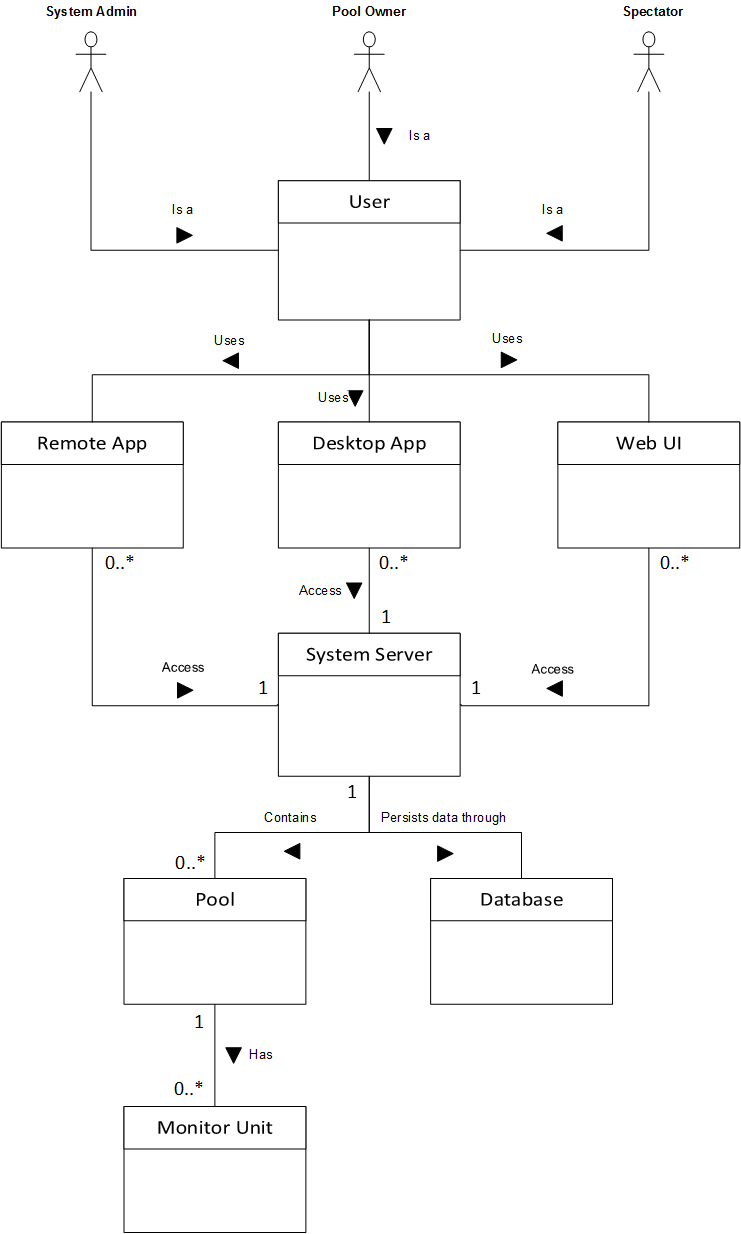
\includegraphics[width=\linewidth]{figs/domainModel}
	\caption{Domænemodel for systemet}
	\label{fig:domainmodel}
\end{figure}

\todo{Fig~\ref{fig:domainmodel} skal beskrives som et ''tidligt design'' eftersom det overhovedet ikke ligner systemet som det er nu. En ny model skal nok laves.}

\subsection{Domænebeskrivelser}
Med udgangspunkt i modellen på figur~\ref{fig:domainmodel} er der opstillet analyser af de enkelte domæner.

\subsubsection{\gls{user}}\todo{Afsnit skal måske rettes lidt...}
\gls{user} er systemet primære bruger. En \gls{user} kan tillade og/eller fjerne \glspl{spectator}. En \gls{user} kan regulere pH/klor/temperatur værdier inden for evt. lovmæssige begrænsninger. Tilføjelse\footnote{Mulighed for tilføjelse af  \gls{mu} giver \gls{user} mulighed for at tilføje flere/større \glspl{pool} og/eller \glspl{mu}.} af \glspl{mu} er \glspl{user} ansvar. En \gls{user} har mulighed for at sende en \gls{specinvite} til en anden \gls{user}. Dette gøres ved at sende et link\footnote{En \gls{user} kan gennem \gls{pcapp} få genereret et link som \gls{user} selv står for at sende.}  til anden partens email-addresse.

\todo{Reference skal muligvis tilføjes.}

\subsubsection{\Gls{spectator}}
En \gls{spectator} er en \gls{user} der med tillladelse fra en anden \gls{user} får mulighed for at se med på dennes pooldata. Hvis den anden \gls{user} har et system bestående af flere \gls{mu}.

\subsubsection{\gls{pcapp}}
\gls{pcapp} primære formål er at gengive pooldata som findes på Databasen. En \gls{user} kan igennem \gls{pcapp}:

\begin{itemize}
	\item Logge ind med personlig brugerprofil.
	\item Generere et link til invitation af \gls{spectator}.
	\item Se grafisk gengivelse af historisk data.
	\item Se nuværende Pool data.
	\item Sætte \gls{tv} for Pool.
	\item Registrere en eller flere \gls{mu}.
\end{itemize}

\subsubsection{\gls{iosapp}}
En \gls{iosapp} er en “lightweight” udgave af \gls{pcapp}. Denne applikations formål er at \gls{user} kan danne sig et overblik over dataen fra de \gls{mu} der er tilknyttet konto.

\subsubsection{NetworkConnection}
Til at transmittere data fra \gls{mu} til Database, samt fra Database til \gls{pcapp} og \gls{iosapp} benyttes en netværksforbindelse.  For at systemet skal fungere er det et krav at både \gls{pcapp} og remote applikation, databaseserver samt \gls{mu}\footnote{\gls{mu} har ikke en direkte forbindelse til internettet, men benytter sig af en endnu ikke defineret mediator.} har forbindelse til internettet.

\subsubsection{\gls{admin}}
En \gls{admin} er en medarbejder fra \gls{smartpool}, og har rettigheder til at fjerne brugere fra systemet. Det er \glspl{admin} ansvar at de lovmæssige standarder \todo{Reference + lovmæssige værdier findes ikke længere i databasen} for pH/klor/varme værdier er defineret i Databasen.

\subsubsection{\gls{db}}
Databasen indeholder brugerdata, såsom brugerens email-adresse, registrerede \gls{mu}, samt måledata. Måledata gemmes i en endnu udefineret tidsperiode, således at \gls{user} har mulighed for at få en grafisk gengivelse\footnote{Evt. Graf, søjlediagram og lign.} af historisk data.

\subsubsection{\gls{mu}}
En \gls{mu} registreres hos \gls{smartpool} gennem \gls{pcapp} applikationen. Med hver \gls{mu} medfølger et serienummer som bruges ved registrering. En \gls{mu} er enheden der måler pH, frit\footnote{Frit klor angriber bakterier, alger og svampeorganismer. Med tiden transformeres frit klor til bunden klor.}\todo{Find reference eller fjern sætning.} klor og total\footnote{Total klor er summen af frit klor og bunden klor.} klor samt varmeværdier i en \gls{pool}. Det er \gls{mu} der står for behandling af rå. Da der er en sammenhæng figur~\ref{fig:chlorinePh} mellem målte pH-værdier og effektivitet af frit klor\todo{reference!} skal den rå data gennemgå en hidtil udefineret matematisk behandling for at kunne vise \gls{user} relevant information. De rå data bruges til at beregne forholdet mellem bunden klor, som er ineffektivt, lugter kraftigt og irriterer øjne\todo{Referencer!} og slimhinder, og frit klor samt \glspl{pool} overordnede sundhedskarakteristika. \gls{mu} ansvar er således:

\paragraph{Måling af data}
\begin{itemize}
	\item Måling af total klor.
	\item Måling frit klor.
	\item Måling af pH-værdi.
	\item Måling af Temperatur.
\end{itemize}

\paragraph{Behandling af rå data}
\begin{itemize}
	\item Beregning af bunden klor.
	\item Beregning af klor der bør tilføres/fjernes fra \gls{pool}.
	\item Beregning af den mængde syre/base der skal tilføres \gls{pool}.
\end{itemize}

\begin{figure}
	\centering
	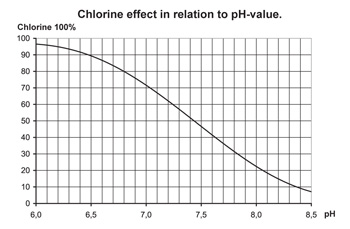
\includegraphics[width=0.7\linewidth]{figs/chlorinePh.png}
	\caption{Sammenhæng mellem effektivitet af frit klor og pH værdi. Kilde: \url{http://www.pahlen.com/users-guide/ph-and-chlorine}}
	\label{fig:chlorinePh}
\end{figure}


\subsubsection{\gls{pool}}
Pool er den enhed der males på. En Pool kan være af hvilken som helst størrelse og form. Hver Pool kan associeres med en \gls{mu}.